\section{Parameterization Methods}


This package provides a second \ccc{parameterize()} entry point
where the user can specify a parameterization method:

\ccFunction{Parameterizer_traits_3<ParameterizationMesh_3>::Error_code parameterize (ParameterizationMesh_3 * mesh, ParameterizerTraits_3 parameterizer);}
{
Compute a 1 to 1 mapping from a triangular 3D surface 'mesh' to a piece of the 2D space. The mapping is linear by pieces (linear in each triangle). The result is the (u,v) pair image of each vertex of the 3D surface.
1 to 1 mapping may be guaranteed or not, depending of ParametizerTraits\_3 algorithm chosen.
Preconditions:\begin{itemize}
\item 'mesh' must be a surface with 1 connected component.\item 'mesh' must be a triangular mesh.\item the mesh border must be mapped onto a convex polygon (for fixed border parameterizations).\end{itemize}
}


This \cgal\ package implements some of the state-of-the-art surface
parameterization methods as models of the \ccc{ParameterizerTraits_3} concept.

This package implements classic border parameterization methods
as models of the \ccc{BorderParameterizer_3} concept. They are used as traits classes
modifying the behavior of the surface parameterization methods.


\subsection{Fixed Border Parameterizations}

\begin{itemize}

\item Tutte Barycentric Mapping \cite{cgal:fh-survey-05}.
One-to-one mapping is guaranteed for convex border.

\ccc{CGAL::Barycentric_mapping_parameterizer_3}  \\

\item Floater Mean Value Coordinates \cite{cgal:f-mvc-03}.
One-to-one mapping is guaranteed for convex border.

\ccc{CGAL::Mean_value_coordinates_parameterizer_3}  \\

\item Discrete Conformal Map \cite{cgal:fh-survey-05}.
Conditionally guaranteed if all weights are positive and border is convex.

\ccc{CGAL::Discrete_conformal_map_parameterizer_3}  \\

\item Discrete Authalic parameterization \cite{cgal:dma-ipsm-02}.
Conditionally guaranteed if all weights are positive and border is convex.

\ccc{CGAL::Discrete_authalic_parameterizer_3}  \\

\end{itemize}

Associated Border Parameterization methods define a
set of constraints: two u,v coordinates for
each instance of a vertex along the border.

\begin{itemize}

\item the user can select a border
    parameterization among two common methods: uniform or
    arc-length parameterization.

\item one convex shape specified by:

    \begin{itemize}

    \item one shape among a set of standard ones (circle, square).

    \item a convex polygon.

    (not yet implemented)

    \end{itemize}

\end{itemize}

\ccc{CGAL::Circular_border_arc_length_parameterizer_3}  \\
\ccc{CGAL::Circular_border_uniform_parameterizer_3}  \\
\ccc{CGAL::Square_border_arc_length_parameterizer_3}  \\
\ccc{CGAL::Square_border_uniform_parameterizer_3}  \\


\subsection{Free Border Parameterizations}

\begin{itemize}

\item Least Squares Conformal Maps \cite{cgal:lprm-lscm-02}.

\ccc{CGAL::LSCM_parameterizer_3}  \\

\item Natural Conformal Map \cite{cgal:dma-ipsm-02}.

(not yet implemented)

\end{itemize}

\begin{itemize}

\item The associated Border Parameterization method define only two constraints (the pinned
vertices). They have to be on the specified border.

\ccc{CGAL::Two_vertices_parameterizer_3}  \\

\end{itemize}


\subsection{Discrete Authalic Parameterization Example}

The code below applies a Discrete Authalic parameterization to a \ccc{Polyhedron_3} mesh:

\begin{ccExampleCode}

// CGAL kernel
typedef CGAL::Cartesian<double>                         Kernel;

// Mesh true type and parameterization adaptors
typedef CGAL::Polyhedron_3<Kernel>                      Polyhedron;
typedef CGAL::Parameterization_polyhedron_adaptor_3<Polyhedron>     
                                                        Parameterization_polyhedron_adaptor;

// Discrete Authalic Parameterization
typedef CGAL::Discrete_authalic_parameterizer_3<Parameterization_polyhedron_adaptor>
                                                        Parameterizer;

int main(int argc,char * argv[])
{
    Polyhedron mesh;
    ...

    // The parameterization package needs an adaptor to handle Polyhedron_3 meshes
    Parameterization_polyhedron_adaptor mesh_adaptor(&mesh);

    // Discrete Authalic Parameterization
    Parameterizer::Error_code err = CGAL::parameterize(&mesh_adaptor, Parameterizer());
    ...
}

\end{ccExampleCode}

See the complete code in \ccc{Authalic_parameterization.C} example.

% Include authalic.png/eps figure with title = "Discrete Authalic Parameterization"
\begin{figure}[bht]
    \begin{center}
        % Image
        \begin{ccTexOnly}
            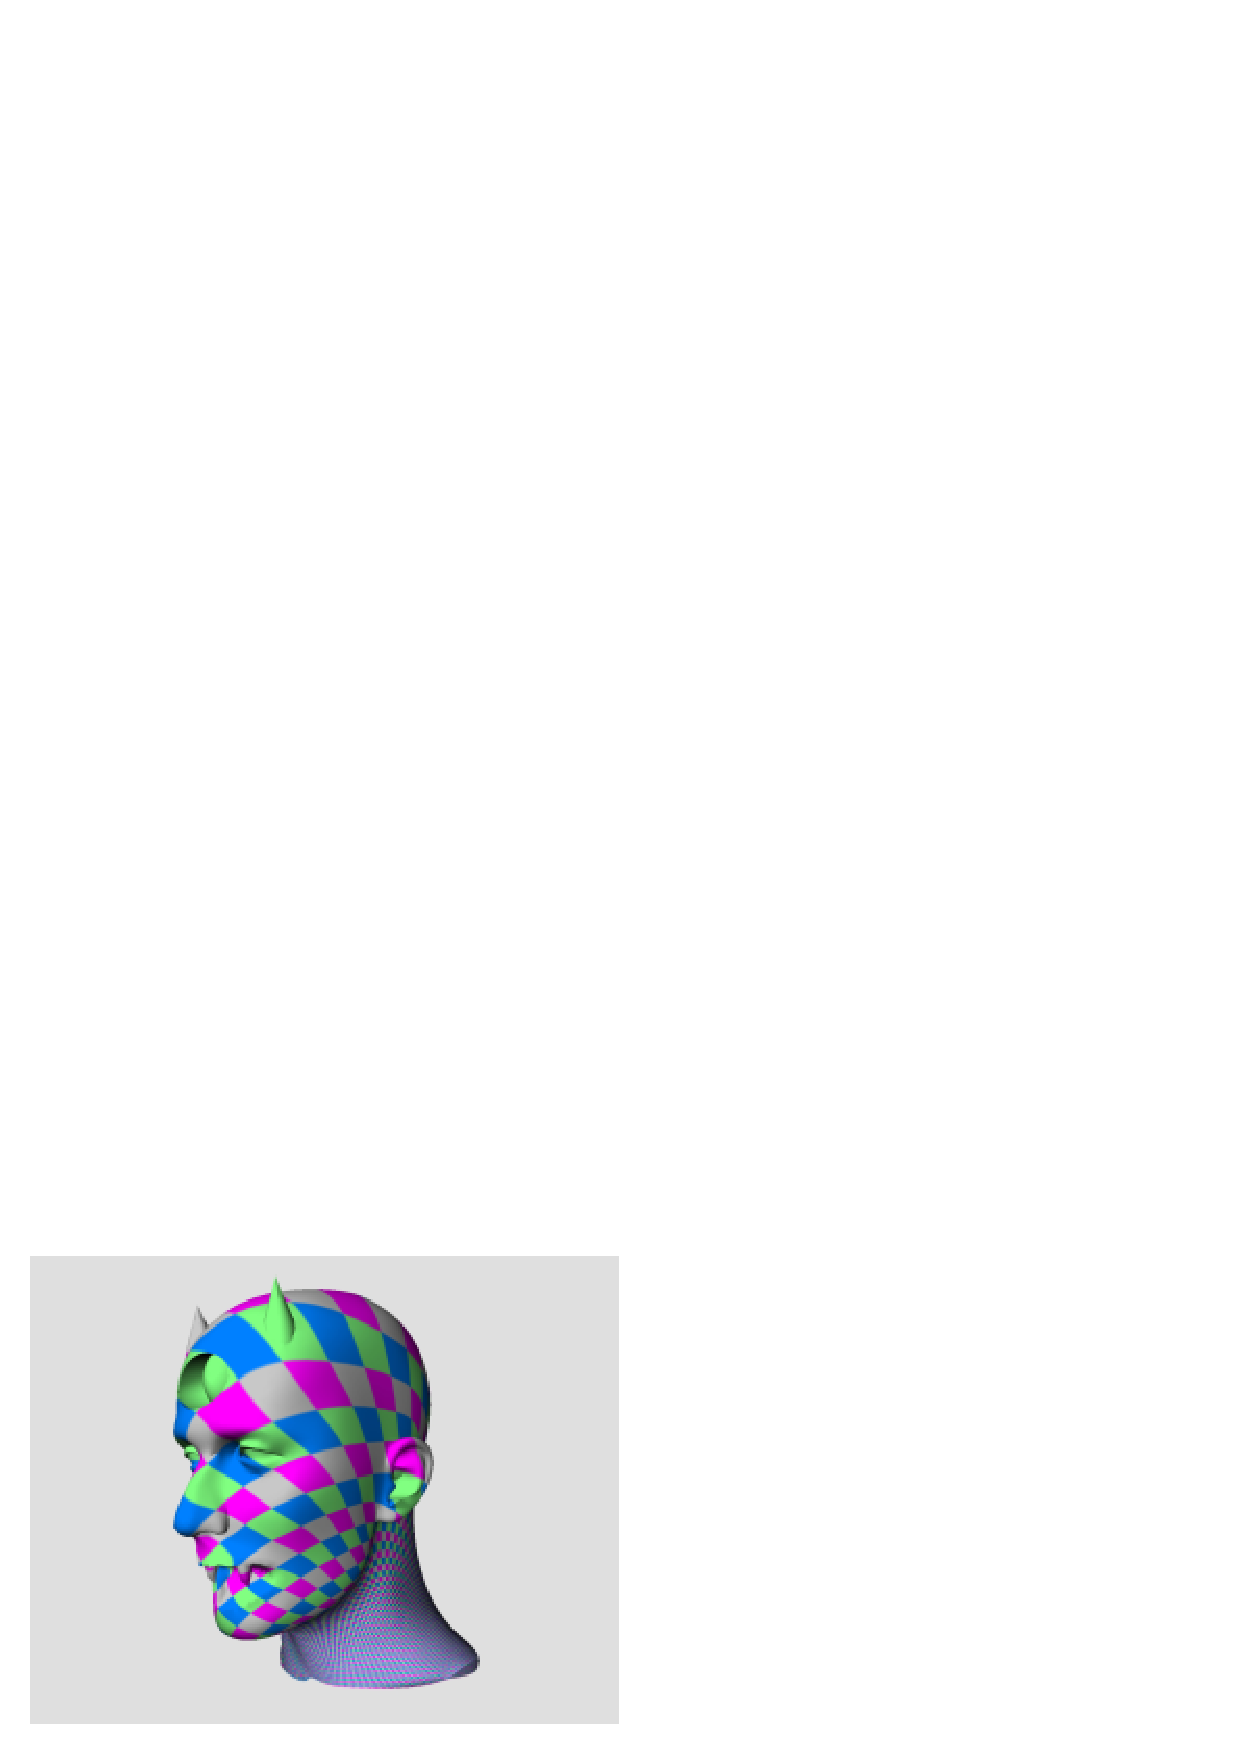
\includegraphics{Parameterization/authalic} % omit suffix to support PS and PDF
        \end{ccTexOnly}
        \begin{ccHtmlOnly}
            <img border=0 src="./authalic.png" align=center>
        \end{ccHtmlOnly}
        \label{parameterization-fig-authalic}

        % Title
        \caption{Discrete Authalic Parameterization}
    \end{center}
\end{figure}


\subsection{Square Border Arc Length Parameterization Example}

The code below applies a Floater Mean Value Coordinates parameterization
with a Square Border Arc Length parameterization:

\begin{ccExampleCode}

// CGAL kernel
typedef CGAL::Cartesian<double>                         Kernel;

// Mesh true type and parameterization adaptors
typedef CGAL::Polyhedron_3<Kernel>                      Polyhedron;
typedef CGAL::Parameterization_polyhedron_adaptor_3<Polyhedron>     
                                                        Parameterization_polyhedron_adaptor;

// Square border parameterizer
typedef CGAL::Square_border_arc_length_parameterizer_3<Parameterization_polyhedron_adaptor>
                                                       Border_parameterizer;

// Floater Mean Value Coordinates parameterizer with square border
typedef CGAL::Mean_value_coordinates_parameterizer_3<Parameterization_polyhedron_adaptor,
                                                     Border_parameterizer>
                                                        Parameterizer;

int main(int argc,char * argv[])
{
    Polyhedron mesh;
    ...

    // The parameterization package needs an adaptor to handle Polyhedron_3 meshes
    Parameterization_polyhedron_adaptor mesh_adaptor(&mesh);

    // Floater Mean Value Coordinates parameterization
    // with a Square Border Arc Length Parameterization
    Parameterizer::Error_code err = CGAL::parameterize(&mesh_adaptor, Parameterizer());
    ...
}

\end{ccExampleCode}

See the complete code in \ccc{Square_border_parameterization.C} example.
